% Options for packages loaded elsewhere
\PassOptionsToPackage{unicode}{hyperref}
\PassOptionsToPackage{hyphens}{url}
\PassOptionsToPackage{dvipsnames,svgnames,x11names}{xcolor}
%
\documentclass[
  letterpaper,
  DIV=11,
  numbers=noendperiod]{scrartcl}

\usepackage{amsmath,amssymb}
\usepackage{lmodern}
\usepackage{iftex}
\ifPDFTeX
  \usepackage[T1]{fontenc}
  \usepackage[utf8]{inputenc}
  \usepackage{textcomp} % provide euro and other symbols
\else % if luatex or xetex
  \usepackage{unicode-math}
  \defaultfontfeatures{Scale=MatchLowercase}
  \defaultfontfeatures[\rmfamily]{Ligatures=TeX,Scale=1}
\fi
% Use upquote if available, for straight quotes in verbatim environments
\IfFileExists{upquote.sty}{\usepackage{upquote}}{}
\IfFileExists{microtype.sty}{% use microtype if available
  \usepackage[]{microtype}
  \UseMicrotypeSet[protrusion]{basicmath} % disable protrusion for tt fonts
}{}
\makeatletter
\@ifundefined{KOMAClassName}{% if non-KOMA class
  \IfFileExists{parskip.sty}{%
    \usepackage{parskip}
  }{% else
    \setlength{\parindent}{0pt}
    \setlength{\parskip}{6pt plus 2pt minus 1pt}}
}{% if KOMA class
  \KOMAoptions{parskip=half}}
\makeatother
\usepackage{xcolor}
\setlength{\emergencystretch}{3em} % prevent overfull lines
\setcounter{secnumdepth}{-\maxdimen} % remove section numbering
% Make \paragraph and \subparagraph free-standing
\ifx\paragraph\undefined\else
  \let\oldparagraph\paragraph
  \renewcommand{\paragraph}[1]{\oldparagraph{#1}\mbox{}}
\fi
\ifx\subparagraph\undefined\else
  \let\oldsubparagraph\subparagraph
  \renewcommand{\subparagraph}[1]{\oldsubparagraph{#1}\mbox{}}
\fi

\usepackage{color}
\usepackage{fancyvrb}
\newcommand{\VerbBar}{|}
\newcommand{\VERB}{\Verb[commandchars=\\\{\}]}
\DefineVerbatimEnvironment{Highlighting}{Verbatim}{commandchars=\\\{\}}
% Add ',fontsize=\small' for more characters per line
\usepackage{framed}
\definecolor{shadecolor}{RGB}{241,243,245}
\newenvironment{Shaded}{\begin{snugshade}}{\end{snugshade}}
\newcommand{\AlertTok}[1]{\textcolor[rgb]{0.68,0.00,0.00}{#1}}
\newcommand{\AnnotationTok}[1]{\textcolor[rgb]{0.37,0.37,0.37}{#1}}
\newcommand{\AttributeTok}[1]{\textcolor[rgb]{0.40,0.45,0.13}{#1}}
\newcommand{\BaseNTok}[1]{\textcolor[rgb]{0.68,0.00,0.00}{#1}}
\newcommand{\BuiltInTok}[1]{\textcolor[rgb]{0.00,0.23,0.31}{#1}}
\newcommand{\CharTok}[1]{\textcolor[rgb]{0.13,0.47,0.30}{#1}}
\newcommand{\CommentTok}[1]{\textcolor[rgb]{0.37,0.37,0.37}{#1}}
\newcommand{\CommentVarTok}[1]{\textcolor[rgb]{0.37,0.37,0.37}{\textit{#1}}}
\newcommand{\ConstantTok}[1]{\textcolor[rgb]{0.56,0.35,0.01}{#1}}
\newcommand{\ControlFlowTok}[1]{\textcolor[rgb]{0.00,0.23,0.31}{#1}}
\newcommand{\DataTypeTok}[1]{\textcolor[rgb]{0.68,0.00,0.00}{#1}}
\newcommand{\DecValTok}[1]{\textcolor[rgb]{0.68,0.00,0.00}{#1}}
\newcommand{\DocumentationTok}[1]{\textcolor[rgb]{0.37,0.37,0.37}{\textit{#1}}}
\newcommand{\ErrorTok}[1]{\textcolor[rgb]{0.68,0.00,0.00}{#1}}
\newcommand{\ExtensionTok}[1]{\textcolor[rgb]{0.00,0.23,0.31}{#1}}
\newcommand{\FloatTok}[1]{\textcolor[rgb]{0.68,0.00,0.00}{#1}}
\newcommand{\FunctionTok}[1]{\textcolor[rgb]{0.28,0.35,0.67}{#1}}
\newcommand{\ImportTok}[1]{\textcolor[rgb]{0.00,0.46,0.62}{#1}}
\newcommand{\InformationTok}[1]{\textcolor[rgb]{0.37,0.37,0.37}{#1}}
\newcommand{\KeywordTok}[1]{\textcolor[rgb]{0.00,0.23,0.31}{#1}}
\newcommand{\NormalTok}[1]{\textcolor[rgb]{0.00,0.23,0.31}{#1}}
\newcommand{\OperatorTok}[1]{\textcolor[rgb]{0.37,0.37,0.37}{#1}}
\newcommand{\OtherTok}[1]{\textcolor[rgb]{0.00,0.23,0.31}{#1}}
\newcommand{\PreprocessorTok}[1]{\textcolor[rgb]{0.68,0.00,0.00}{#1}}
\newcommand{\RegionMarkerTok}[1]{\textcolor[rgb]{0.00,0.23,0.31}{#1}}
\newcommand{\SpecialCharTok}[1]{\textcolor[rgb]{0.37,0.37,0.37}{#1}}
\newcommand{\SpecialStringTok}[1]{\textcolor[rgb]{0.13,0.47,0.30}{#1}}
\newcommand{\StringTok}[1]{\textcolor[rgb]{0.13,0.47,0.30}{#1}}
\newcommand{\VariableTok}[1]{\textcolor[rgb]{0.07,0.07,0.07}{#1}}
\newcommand{\VerbatimStringTok}[1]{\textcolor[rgb]{0.13,0.47,0.30}{#1}}
\newcommand{\WarningTok}[1]{\textcolor[rgb]{0.37,0.37,0.37}{\textit{#1}}}

\providecommand{\tightlist}{%
  \setlength{\itemsep}{0pt}\setlength{\parskip}{0pt}}\usepackage{longtable,booktabs,array}
\usepackage{calc} % for calculating minipage widths
% Correct order of tables after \paragraph or \subparagraph
\usepackage{etoolbox}
\makeatletter
\patchcmd\longtable{\par}{\if@noskipsec\mbox{}\fi\par}{}{}
\makeatother
% Allow footnotes in longtable head/foot
\IfFileExists{footnotehyper.sty}{\usepackage{footnotehyper}}{\usepackage{footnote}}
\makesavenoteenv{longtable}
\usepackage{graphicx}
\makeatletter
\def\maxwidth{\ifdim\Gin@nat@width>\linewidth\linewidth\else\Gin@nat@width\fi}
\def\maxheight{\ifdim\Gin@nat@height>\textheight\textheight\else\Gin@nat@height\fi}
\makeatother
% Scale images if necessary, so that they will not overflow the page
% margins by default, and it is still possible to overwrite the defaults
% using explicit options in \includegraphics[width, height, ...]{}
\setkeys{Gin}{width=\maxwidth,height=\maxheight,keepaspectratio}
% Set default figure placement to htbp
\makeatletter
\def\fps@figure{htbp}
\makeatother

\usepackage{amsmath}
\KOMAoption{captions}{tableheading}
\makeatletter
\makeatother
\makeatletter
\makeatother
\makeatletter
\@ifpackageloaded{caption}{}{\usepackage{caption}}
\AtBeginDocument{%
\ifdefined\contentsname
  \renewcommand*\contentsname{Table of contents}
\else
  \newcommand\contentsname{Table of contents}
\fi
\ifdefined\listfigurename
  \renewcommand*\listfigurename{List of Figures}
\else
  \newcommand\listfigurename{List of Figures}
\fi
\ifdefined\listtablename
  \renewcommand*\listtablename{List of Tables}
\else
  \newcommand\listtablename{List of Tables}
\fi
\ifdefined\figurename
  \renewcommand*\figurename{Figure}
\else
  \newcommand\figurename{Figure}
\fi
\ifdefined\tablename
  \renewcommand*\tablename{Table}
\else
  \newcommand\tablename{Table}
\fi
}
\@ifpackageloaded{float}{}{\usepackage{float}}
\floatstyle{ruled}
\@ifundefined{c@chapter}{\newfloat{codelisting}{h}{lop}}{\newfloat{codelisting}{h}{lop}[chapter]}
\floatname{codelisting}{Listing}
\newcommand*\listoflistings{\listof{codelisting}{List of Listings}}
\makeatother
\makeatletter
\@ifpackageloaded{caption}{}{\usepackage{caption}}
\@ifpackageloaded{subcaption}{}{\usepackage{subcaption}}
\makeatother
\makeatletter
\@ifpackageloaded{tcolorbox}{}{\usepackage[many]{tcolorbox}}
\makeatother
\makeatletter
\@ifundefined{shadecolor}{\definecolor{shadecolor}{rgb}{.97, .97, .97}}
\makeatother
\makeatletter
\makeatother
\ifLuaTeX
  \usepackage{selnolig}  % disable illegal ligatures
\fi
\IfFileExists{bookmark.sty}{\usepackage{bookmark}}{\usepackage{hyperref}}
\IfFileExists{xurl.sty}{\usepackage{xurl}}{} % add URL line breaks if available
\urlstyle{same} % disable monospaced font for URLs
\hypersetup{
  pdftitle={STAT 631 Homework 1},
  pdfauthor={Jack Cunningham (jgavc@tamu.edu)},
  colorlinks=true,
  linkcolor={blue},
  filecolor={Maroon},
  citecolor={Blue},
  urlcolor={Blue},
  pdfcreator={LaTeX via pandoc}}

\title{STAT 631 Homework 1}
\author{Jack Cunningham (jgavc@tamu.edu)}
\date{9/3/24}

\begin{document}
\maketitle
\ifdefined\Shaded\renewenvironment{Shaded}{\begin{tcolorbox}[borderline west={3pt}{0pt}{shadecolor}, enhanced, sharp corners, interior hidden, frame hidden, boxrule=0pt, breakable]}{\end{tcolorbox}}\fi

1)

\begin{Shaded}
\begin{Highlighting}[]
\FunctionTok{set.seed}\NormalTok{(}\DecValTok{2012}\NormalTok{)}
\NormalTok{n }\OtherTok{=} \DecValTok{253}
\FunctionTok{par}\NormalTok{(}\AttributeTok{mfrow =} \FunctionTok{c}\NormalTok{(}\DecValTok{3}\NormalTok{,}\DecValTok{3}\NormalTok{))}
\ControlFlowTok{for}\NormalTok{ (i }\ControlFlowTok{in}\NormalTok{ (}\DecValTok{1}\SpecialCharTok{:}\DecValTok{9}\NormalTok{))\{}
\NormalTok{  logr }\OtherTok{=} \FunctionTok{rnorm}\NormalTok{(n, }\FloatTok{0.05}\SpecialCharTok{/}\DecValTok{253}\NormalTok{, }\FloatTok{0.2}\SpecialCharTok{/}\FunctionTok{sqrt}\NormalTok{(}\DecValTok{253}\NormalTok{))}
\NormalTok{  price }\OtherTok{=} \FunctionTok{c}\NormalTok{(}\DecValTok{120}\NormalTok{, }\DecValTok{120} \SpecialCharTok{*} \FunctionTok{exp}\NormalTok{(}\FunctionTok{cumsum}\NormalTok{(logr)))}
  \FunctionTok{plot}\NormalTok{(price, }\AttributeTok{type =} \StringTok{"l"}\NormalTok{)}
\NormalTok{\}}
\end{Highlighting}
\end{Shaded}

\begin{figure}[H]

{\centering 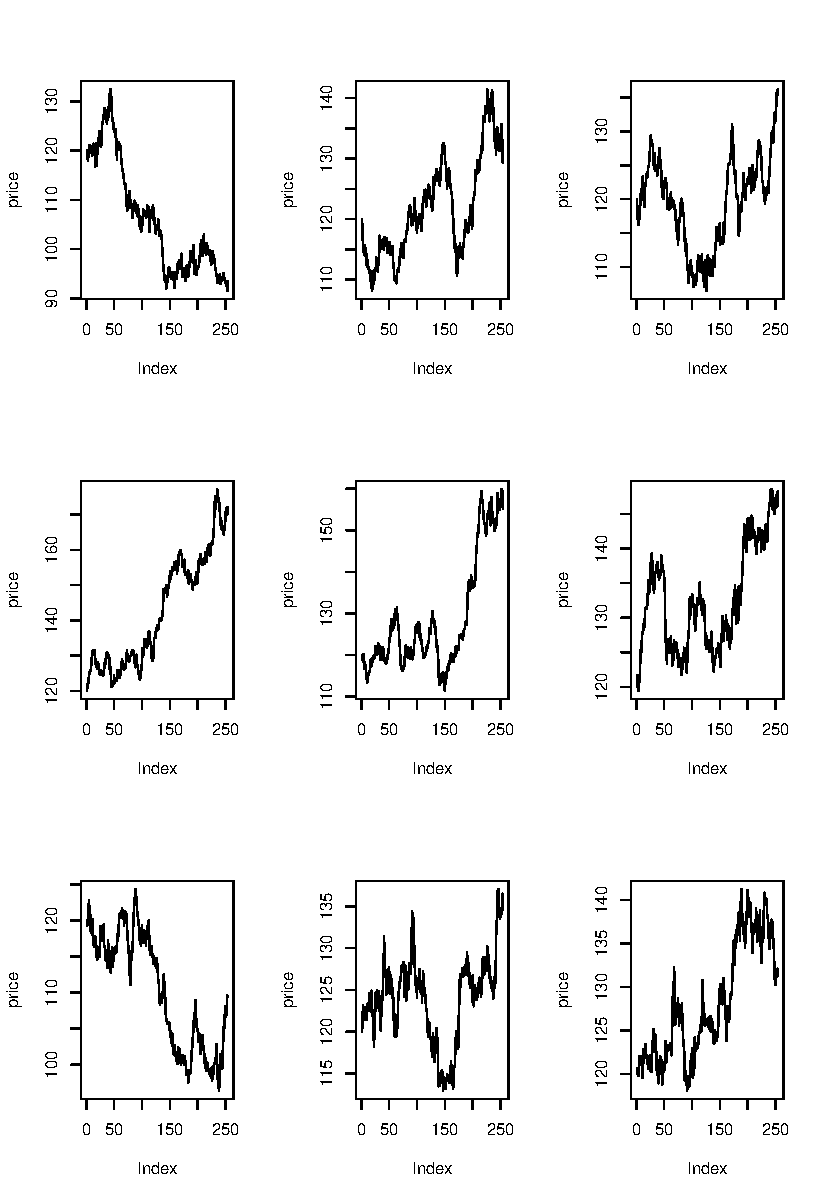
\includegraphics{homework_1_files/figure-pdf/unnamed-chunk-1-1.pdf}

}

\end{figure}

Problem 9)

We are generating the daily log-return data by using a normal
distribution with parameters \(\mu=\frac{0.05}{253}\) and
\(\sigma=\frac{0.2}{\sqrt{253}}\). Thus for a one year period (with 253
trading days) the mean of the log-return is
\(\mu t=\frac{0.05}{253}(253)=0.05\) and the standard deviation is
\(\sigma\sqrt{t}=\frac{0.2}{\sqrt{253}}(\sqrt{253})=0.2\).

Problem 10)

We can see many clumps of time where it appears positive (negative)
returns are followed by positive (negative) returns. In this case we are
sure that this appearance of momentum is an illusion since we generated
this simulation with i.i.d log-returns. In other words each day's return
was independent and was not impacted by the previous days.

Problem 11)

First we have the c() function which serves to concatenate vectors. Its
first entry is the initial price of the asset, 120. Its second entry is
a bit more involved. The variable logr has each days generated log
return. The cumsum function creates a cumulative summation of the vector
logr. This allows us to track the log return as it moves over time. We
take constant \(e\) and raise it by the cumulative log return to bring
us back to the cumulative return. We then multiply by 120 to get the
prices for each day.

2.

Problem 17)\\

\begin{Shaded}
\begin{Highlighting}[]
\NormalTok{data }\OtherTok{=} \FunctionTok{read.csv}\NormalTok{(}\StringTok{\textquotesingle{}MCD\_PriceDaily.csv\textquotesingle{}}\NormalTok{)}
\NormalTok{logReturn }\OtherTok{=} \FunctionTok{diff}\NormalTok{(}\FunctionTok{log}\NormalTok{(data[,}\StringTok{"Adj.Close"}\NormalTok{]))}
\FunctionTok{head}\NormalTok{(logReturn)}
\end{Highlighting}
\end{Shaded}

\begin{verbatim}
[1] -0.0076229801 -0.0137181518  0.0073522812 -0.0009395848  0.0076786593
[6]  0.0053958639
\end{verbatim}

\begin{Shaded}
\begin{Highlighting}[]
\CommentTok{\#Simulation of situation}
\NormalTok{niter }\OtherTok{=} \DecValTok{10000}
\FunctionTok{set.seed}\NormalTok{(}\DecValTok{2015}\NormalTok{)}
\NormalTok{outcome }\OtherTok{=} \FunctionTok{rep}\NormalTok{(}\DecValTok{0}\NormalTok{, niter)}

\ControlFlowTok{for}\NormalTok{(i }\ControlFlowTok{in}\NormalTok{ (}\DecValTok{1}\SpecialCharTok{:}\NormalTok{niter))\{}
\NormalTok{  logr }\OtherTok{=} \FunctionTok{rnorm}\NormalTok{(}\DecValTok{20}\NormalTok{, }\AttributeTok{mean =} \FunctionTok{mean}\NormalTok{(logReturn), }\AttributeTok{sd =} \FunctionTok{sd}\NormalTok{(logReturn))}
\NormalTok{  price }\OtherTok{=} \FloatTok{93.07}\SpecialCharTok{*}\FunctionTok{exp}\NormalTok{(}\FunctionTok{cumsum}\NormalTok{(logr))}
  
  \CommentTok{\#Boolean with check to see if price went under 84.5}
\NormalTok{  outcome[i] }\OtherTok{=} \FunctionTok{ifelse}\NormalTok{(}\FunctionTok{sum}\NormalTok{(price }\SpecialCharTok{\textless{}} \FloatTok{84.5}\NormalTok{) }\SpecialCharTok{\textgreater{}=} \DecValTok{1}\NormalTok{, }\DecValTok{125}\NormalTok{, }\SpecialCharTok{{-}}\DecValTok{1}\NormalTok{)}
  
\NormalTok{\}}
\end{Highlighting}
\end{Shaded}

\begin{Shaded}
\begin{Highlighting}[]
\CommentTok{\#Expected Value from Bet}
\NormalTok{ev }\OtherTok{\textless{}{-}} \FunctionTok{mean}\NormalTok{(outcome)}
\NormalTok{s }\OtherTok{\textless{}{-}} \FunctionTok{sd}\NormalTok{(outcome)}
\NormalTok{lower }\OtherTok{\textless{}{-}}\NormalTok{ ev }\SpecialCharTok{{-}} \FunctionTok{qt}\NormalTok{(.}\DecValTok{975}\NormalTok{,}\AttributeTok{df =}\NormalTok{ niter }\SpecialCharTok{{-}} \DecValTok{1}\NormalTok{)}\SpecialCharTok{*}\NormalTok{s}\SpecialCharTok{/}\FunctionTok{sqrt}\NormalTok{(niter)}
\NormalTok{upper }\OtherTok{\textless{}{-}}\NormalTok{ ev }\SpecialCharTok{+} \FunctionTok{qt}\NormalTok{(.}\DecValTok{975}\NormalTok{,}\AttributeTok{df =}\NormalTok{ niter }\SpecialCharTok{{-}} \DecValTok{1}\NormalTok{)}\SpecialCharTok{*}\NormalTok{s}\SpecialCharTok{/}\FunctionTok{sqrt}\NormalTok{(niter)}
\NormalTok{ev}
\end{Highlighting}
\end{Shaded}

\begin{verbatim}
[1] -0.0802
\end{verbatim}

\begin{Shaded}
\begin{Highlighting}[]
\FunctionTok{c}\NormalTok{(lower,upper)}
\end{Highlighting}
\end{Shaded}

\begin{verbatim}
[1] -0.2904632  0.1300632
\end{verbatim}

The expected value from the bet is -0.0802 with a confidence interval of
(-0.29, 0.13). With this information I would avoid taking this bet.

3)

a)

Log-returns are normally distributed with parameters
\(\mu = 0.001, \sigma = 0.015\).

We know:

\(\log(P_1)=\log(P_0)+\log(1 + R_1(t))\).

In this case we are looking for the chance of initial price \(P_0=1000\)
dropping to less than \(P_1=990\) in the next day. That is a return of
\(R_1=\frac{990-1000}{1000}=-0.01\). So we need to find the chance of a
\(\log(1 -0.01)=\log(.99)\) move in the log return or less. That is:

\(P[r \leq \log(.99)]=P[r^* \leq \frac{\log(.99)-0.001}{0.015}]\)

\begin{Shaded}
\begin{Highlighting}[]
\NormalTok{Z }\OtherTok{=}\NormalTok{ (}\FunctionTok{log}\NormalTok{(.}\DecValTok{99}\NormalTok{) }\SpecialCharTok{{-}}\NormalTok{ .}\DecValTok{001}\NormalTok{)}\SpecialCharTok{/}\FloatTok{0.015}
\NormalTok{chance }\OtherTok{=} \FunctionTok{pnorm}\NormalTok{(Z)}
\NormalTok{chance}
\end{Highlighting}
\end{Shaded}

\begin{verbatim}
[1] 0.2306557
\end{verbatim}

There is a probability of 0.231 that tomorrow price for this investment
will drop to below \$990.

b)

Since \(r_1,r_2,…r_t\) are i.i.d with a normal distribution. When
\(r_1,r_2,r_3,r_4,r_5\) are added together their cumulative distribution
is \(N(5 \mu,5\sigma^2)\). We have return
\(R_1=\frac{990-1000}{1000}=-0.01\). so we need to find the chance of a
\(\log(1-0.01) = \log(.99)\) move in the log return or less. That is:

\(P[r_5 \leq log(.99)=P[r_5^* \leq\frac{log(.99)-0.001}{0.015\sqrt{5}}]\)

\begin{Shaded}
\begin{Highlighting}[]
\NormalTok{Z }\OtherTok{=}\NormalTok{ (}\FunctionTok{log}\NormalTok{(.}\DecValTok{99}\NormalTok{) }\SpecialCharTok{{-}} \FloatTok{0.001}\NormalTok{)}\SpecialCharTok{/}\NormalTok{(}\FloatTok{0.015}\SpecialCharTok{*}\FunctionTok{sqrt}\NormalTok{(}\DecValTok{5}\NormalTok{))}
\NormalTok{chance }\OtherTok{=} \FunctionTok{pnorm}\NormalTok{(Z)}
\NormalTok{chance}
\end{Highlighting}
\end{Shaded}

\begin{verbatim}
[1] 0.370905
\end{verbatim}

There is a probability of 0.371 that this investment will be worth less
than \$990 after 5 trading days.

4)

Given \(P_1=95,P_2=103,P_3=98\). We need to find \(r_3(2)\).

We know that \(r_t(k)=r_t+r_{t-1}+\dots+r_{t-k+1}\)

And that \(r_t=\log(\frac{P_t}{P_{t-1}})=p_t-p_{t-1}\)

In this case \(t =3\) and \(k=2\). So:

\(r_3(2)=r_3+r_2=\log(\frac{98}{103})+\log(\frac{103}{95})=\log(98)-\log(103)+\log(103)-\log(95)=\log(98)-\log(95)\)

\begin{Shaded}
\begin{Highlighting}[]
\NormalTok{r\_3\_2 }\OtherTok{\textless{}{-}} \FunctionTok{log}\NormalTok{(}\DecValTok{98}\NormalTok{)}\SpecialCharTok{{-}}\FunctionTok{log}\NormalTok{(}\DecValTok{95}\NormalTok{)}
\NormalTok{r\_3\_2}
\end{Highlighting}
\end{Shaded}

\begin{verbatim}
[1] 0.03109059
\end{verbatim}

\(r_3(2)\)=0.03109.

\begin{Shaded}
\begin{Highlighting}[]
\CommentTok{\#Generating Symbols}
\FunctionTok{library}\NormalTok{(quantmod)}
\FunctionTok{getSymbols}\NormalTok{(}\AttributeTok{Symbols =} \FunctionTok{c}\NormalTok{(}\StringTok{"\^{}GSPC"}\NormalTok{,}\StringTok{"CVX"}\NormalTok{,}\StringTok{"AMZN"}\NormalTok{), }
           \AttributeTok{from =} \StringTok{"2005{-}01{-}01"}\NormalTok{, }\AttributeTok{to =} \StringTok{"2024{-}08{-}01"}\NormalTok{)}
\end{Highlighting}
\end{Shaded}

\begin{verbatim}
[1] "GSPC" "CVX"  "AMZN"
\end{verbatim}

\begin{Shaded}
\begin{Highlighting}[]
\CommentTok{\#Getting Adjusted Close}
\NormalTok{SnP\_500\_AC }\OtherTok{\textless{}{-}}\NormalTok{ GSPC[, }\StringTok{"GSPC.Adjusted"}\NormalTok{]}
\NormalTok{Chevron\_AC }\OtherTok{\textless{}{-}}\NormalTok{ CVX[, }\StringTok{"CVX.Adjusted"}\NormalTok{]}
\NormalTok{Amazon\_AC }\OtherTok{\textless{}{-}}\NormalTok{ AMZN[, }\StringTok{"AMZN.Adjusted"}\NormalTok{]}
\end{Highlighting}
\end{Shaded}

\begin{Shaded}
\begin{Highlighting}[]
\CommentTok{\#Getting daily log return}
\NormalTok{SnP\_500\_dlr }\OtherTok{\textless{}{-}} \FunctionTok{dailyReturn}\NormalTok{(SnP\_500\_AC, }\AttributeTok{type =} \StringTok{"log"}\NormalTok{)}
\NormalTok{Chevron\_dlr }\OtherTok{\textless{}{-}} \FunctionTok{dailyReturn}\NormalTok{(Chevron\_AC, }\AttributeTok{type =} \StringTok{"log"}\NormalTok{)}
\NormalTok{Amazon\_dlr }\OtherTok{\textless{}{-}} \FunctionTok{dailyReturn}\NormalTok{(Amazon\_AC, }\AttributeTok{type =} \StringTok{"log"}\NormalTok{)}
\end{Highlighting}
\end{Shaded}

5.

a)

\begin{Shaded}
\begin{Highlighting}[]
\FunctionTok{plot}\NormalTok{(SnP\_500\_AC[}\StringTok{"2018{-}01{-}01::2024{-}8{-}01"}\NormalTok{], }\AttributeTok{main =} \StringTok{"GSPC Stock Price"}\NormalTok{)}
\end{Highlighting}
\end{Shaded}

\begin{figure}[H]

{\centering 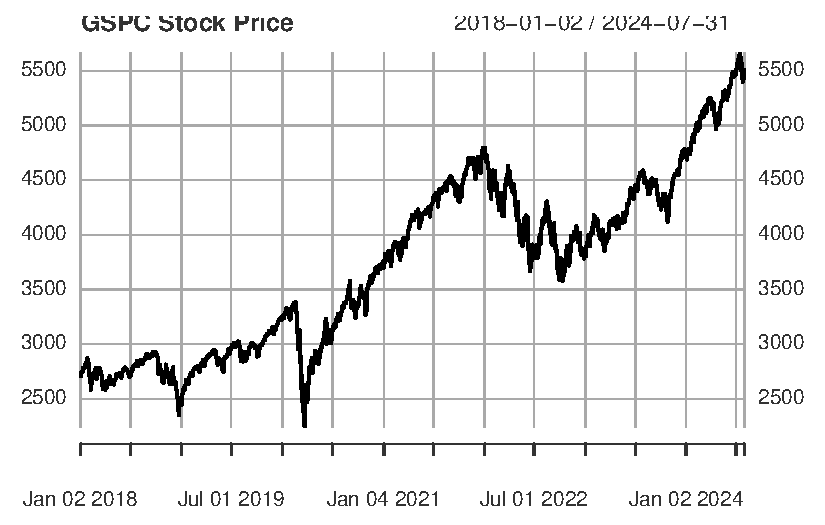
\includegraphics{homework_1_files/figure-pdf/unnamed-chunk-11-1.pdf}

}

\end{figure}

\begin{Shaded}
\begin{Highlighting}[]
\FunctionTok{plot}\NormalTok{(SnP\_500\_dlr[}\StringTok{"2018{-}01{-}01::2024{-}8{-}01"}\NormalTok{], }\AttributeTok{main =} \StringTok{"GSPC Daily Log Return"}\NormalTok{)}
\end{Highlighting}
\end{Shaded}

\begin{figure}[H]

{\centering 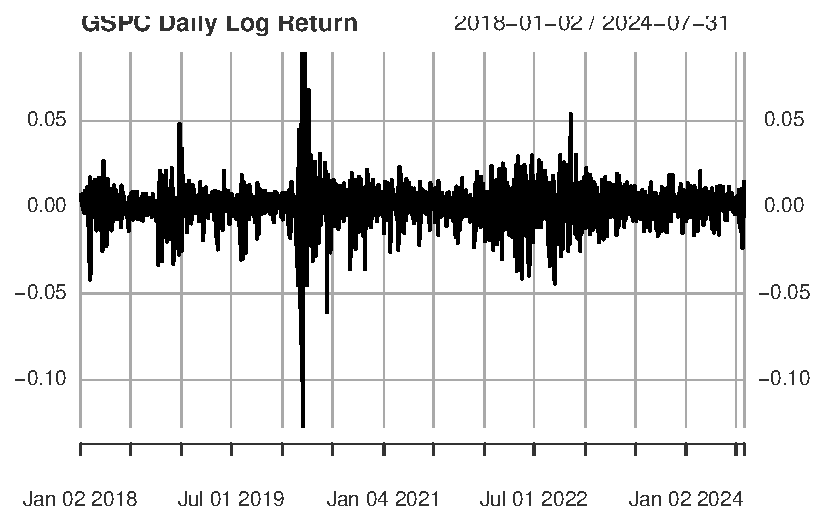
\includegraphics{homework_1_files/figure-pdf/unnamed-chunk-11-2.pdf}

}

\end{figure}

One of the first major events in this time period was the sell off at
the end of 2018. That December there were a few factors that drove
volatility, most importantly in my opinion was a concern about the
stability of the economy as the FED continued raising rates and reducing
their balance sheet after a mediocre November 2018 jobs report. Another
factor that drove a lot of volatility throughout 2018, and much of the
Trump presidency, were the trade and tariff negotiations with China.
There was a ton of action and counteraction between the US and China,
tariffs and counter-tariffs would hit the news, or be tweeted directly
from Trump himself, and cause a flurry of trading action. The reason I
believe the overall economic condition concerns were the primary cause
of the sell-off is because on December 1st 2018 the US and China agreed
on a 90-day halt to new tariffs, seeming to indicate some positive
traction on a trade deal. But it would remiss to not believe it was a
combination of the two.

In August of 2019 there was a lot volatility despite a lack of direction
on the month, this was mainly due to trade tensions between the US and
China and a yield reversion in the bond market causing some recessionary
fears. On August 5th Trump had accused China of currency manipulation
after the yuan steeply fell in value, that day the S\&P 500 dropped
about 3\% fearing a ignition in the trade war.

In Match of 2020 there was COVID-19. A historic amount of uncertainty
was present in the market as investors debated how it would affect the
global economy. Ultimately the recovery after the sell-off was rather
steep.

Throughout 2022 and 2023 the market faced what appeared to be runaway
inflation with CPI peaking at 9.1\% and a new conflict as Russia invaded
Ukraine. The ascent of inflation at this time forced the reluctant FED
into action to begin raising rates. The FED had been consistent about
the theory that inflation was transitory, a temporary blip in prices due
to COVID supply chain disruption. However as 2022 progressed and the CPI
kept hitting new highs the FED had to begin raising the Federal Funds
rate, with 11 hikes between March of 2022 and July of 2023. The federal
funds target went from 0-.25\% to 5.25-5.50\% in that time. At the same
time the Russian invasion of Ukraine heightened the risk of a global
conflict and lead to a realignment in the global economy as west powers
began placing embargoes on Russia. The S\&P would sell off and recover
in 2023 and 2024.

Most recently there was a large amount of volatility at the start of
August 2024. Part of the concern was a bad job report for July, raising
concerns that a weakened job market would wreck the soft landing the FED
has been striving for. Another aspect was a rate hike in Japan, the
first since 2007, and an indication that there may be more hawkish
actions to come. There was a large amount of institutions executing the
``yen carry trade''. The trader would borrow yen for an extremely low
interest rate and buy, for instance, a treasury bill in the US paying
north of 5\%. The trader faces foreign exchange risk in this
transaction, if the value of the yen appreciates relative to the dollar
the amount of yen they have to pay back becomes more expensive to buy.
After the actions taken by the central back in Japan the unwinding of
this transaction arguably caused a lot of volatility in these couple of
days.

b)

\begin{Shaded}
\begin{Highlighting}[]
\FunctionTok{library}\NormalTok{(tidyverse)}
\NormalTok{stock\_data }\OtherTok{\textless{}{-}} \FunctionTok{data.frame}\NormalTok{(}
  \AttributeTok{date =} \FunctionTok{index}\NormalTok{(GSPC),}
  \AttributeTok{SnP\_500\_AD =} \FunctionTok{as.numeric}\NormalTok{(GSPC[, }\StringTok{"GSPC.Adjusted"}\NormalTok{]),}
  \AttributeTok{Chevron\_AD =} \FunctionTok{as.numeric}\NormalTok{(CVX[, }\StringTok{"CVX.Adjusted"}\NormalTok{]),}
  \AttributeTok{Amazon\_AD =} \FunctionTok{as.numeric}\NormalTok{(AMZN[, }\StringTok{"AMZN.Adjusted"}\NormalTok{]),}
  \AttributeTok{SnP\_500\_dlr =} \FunctionTok{as.numeric}\NormalTok{(}\FunctionTok{dailyReturn}\NormalTok{(}\FunctionTok{Ad}\NormalTok{(GSPC), }\AttributeTok{type =} \StringTok{"log"}\NormalTok{)),}
  \AttributeTok{Chevron\_dlr =} \FunctionTok{as.numeric}\NormalTok{(}\FunctionTok{dailyReturn}\NormalTok{(}\FunctionTok{Ad}\NormalTok{(CVX), }\AttributeTok{type =} \StringTok{"log"}\NormalTok{)),}
  \AttributeTok{Amazon\_dlr =} \FunctionTok{as.numeric}\NormalTok{(}\FunctionTok{dailyReturn}\NormalTok{(}\FunctionTok{Ad}\NormalTok{(AMZN)), }\AttributeTok{type =} \StringTok{"log"}\NormalTok{)}
\NormalTok{)}
\end{Highlighting}
\end{Shaded}

\begin{Shaded}
\begin{Highlighting}[]
\FunctionTok{library}\NormalTok{(tidyverse)}
\NormalTok{colors }\OtherTok{\textless{}{-}} \FunctionTok{c}\NormalTok{(}\StringTok{"AMZN"} \OtherTok{=} \StringTok{"\#ff9900"}\NormalTok{, }\StringTok{"CVX"} \OtherTok{=} \StringTok{"\#0050AA"}\NormalTok{)}

\NormalTok{stock\_data }\SpecialCharTok{|\textgreater{}}
  \FunctionTok{filter}\NormalTok{(date }\SpecialCharTok{\textgreater{}} \StringTok{"2018{-}01{-}01"}\NormalTok{) }\SpecialCharTok{|\textgreater{}} 
  \FunctionTok{ggplot}\NormalTok{(}\FunctionTok{aes}\NormalTok{(}\AttributeTok{x =}\NormalTok{ date)) }\SpecialCharTok{+}
  \FunctionTok{geom\_line}\NormalTok{(}\FunctionTok{aes}\NormalTok{(}\AttributeTok{y =}\NormalTok{ Chevron\_AD, }\AttributeTok{color =} \StringTok{"CVX"}\NormalTok{)) }\SpecialCharTok{+}
  \FunctionTok{geom\_line}\NormalTok{(}\FunctionTok{aes}\NormalTok{(}\AttributeTok{y =}\NormalTok{ Amazon\_AD, }\AttributeTok{color =} \StringTok{"AMZN"}\NormalTok{)) }\SpecialCharTok{+}
  \FunctionTok{labs}\NormalTok{(}\AttributeTok{title =} \StringTok{"CVX and AMZN Stock Prices"}\NormalTok{, }\AttributeTok{x =} \StringTok{"Date"}\NormalTok{, }\AttributeTok{y =} \StringTok{"price"}\NormalTok{, }
       \AttributeTok{color =} \StringTok{"Legend"}\NormalTok{) }\SpecialCharTok{+}
  \FunctionTok{scale\_color\_manual}\NormalTok{(}\AttributeTok{values =}\NormalTok{ colors)}
\end{Highlighting}
\end{Shaded}

\begin{figure}[H]

{\centering 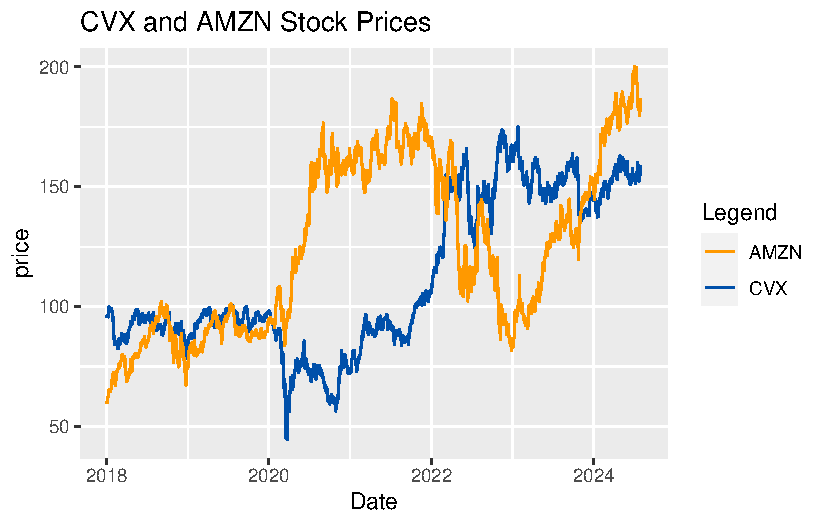
\includegraphics{homework_1_files/figure-pdf/unnamed-chunk-13-1.pdf}

}

\end{figure}

\begin{Shaded}
\begin{Highlighting}[]
\NormalTok{stock\_data }\SpecialCharTok{|\textgreater{}}
  \FunctionTok{filter}\NormalTok{(date }\SpecialCharTok{\textgreater{}} \StringTok{"2018{-}01{-}01"}\NormalTok{) }\SpecialCharTok{|\textgreater{}} 
  \FunctionTok{ggplot}\NormalTok{(}\FunctionTok{aes}\NormalTok{(}\AttributeTok{x =}\NormalTok{ date)) }\SpecialCharTok{+}
  \FunctionTok{geom\_line}\NormalTok{(}\FunctionTok{aes}\NormalTok{(}\AttributeTok{y =}\NormalTok{ Chevron\_dlr, }\AttributeTok{color =} \StringTok{"CVX"}\NormalTok{)) }\SpecialCharTok{+}
  \FunctionTok{geom\_line}\NormalTok{(}\FunctionTok{aes}\NormalTok{(}\AttributeTok{y =}\NormalTok{ Amazon\_dlr, }\AttributeTok{color =} \StringTok{"AMZN"}\NormalTok{), }\AttributeTok{alpha =} \FloatTok{0.8}\NormalTok{) }\SpecialCharTok{+}
  \FunctionTok{labs}\NormalTok{(}\AttributeTok{title =} \StringTok{"CVX and AMZN Daily Log Return"}\NormalTok{, }\AttributeTok{x =} \StringTok{"Date"}\NormalTok{, }\AttributeTok{y =} \StringTok{"Log Return"}\NormalTok{, }
       \AttributeTok{color =} \StringTok{"Legend"}\NormalTok{) }\SpecialCharTok{+}
  \FunctionTok{scale\_color\_manual}\NormalTok{(}\AttributeTok{values =}\NormalTok{ colors)}
\end{Highlighting}
\end{Shaded}

\begin{figure}[H]

{\centering 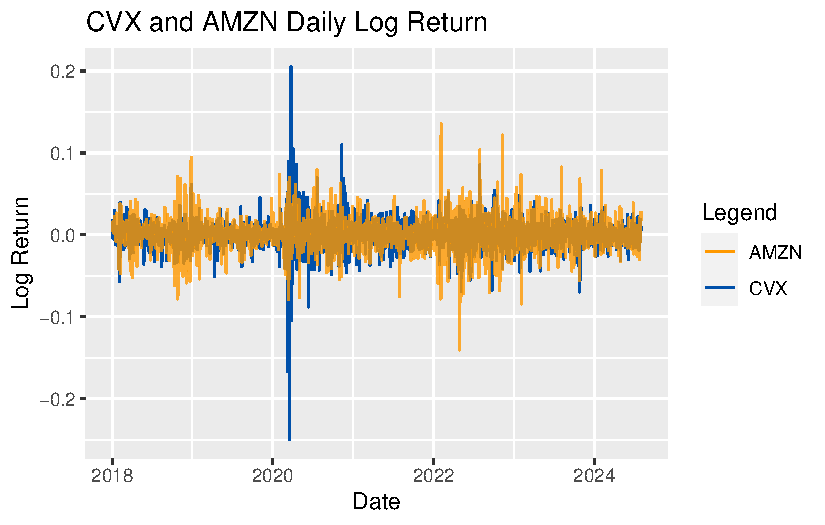
\includegraphics{homework_1_files/figure-pdf/unnamed-chunk-14-1.pdf}

}

\end{figure}

The most striking impact to compare these two stocks is their
performance in the COVID pandemic. Just by taking a look at the daily
log return graph we can see the huge volatility at the start of the
pandemic for Chevron while Amazon's was much more muted compared to
Chevron and the overall market. Chevron is an energy corporation who
fracks and produces oil and gas, and naturally is very exposed to the
demand shrinking as it did under lock-downs in the early pandemic.
Amazon on the other hand thrived in the lock-down era as many consumers
preferred to order their essentials online instead of venturing into a
store.

6)

a)

\begin{Shaded}
\begin{Highlighting}[]
\NormalTok{CVX\_returns }\OtherTok{\textless{}{-}} \FunctionTok{list}\NormalTok{(}
  \AttributeTok{daily =} \FunctionTok{dailyReturn}\NormalTok{(}\FunctionTok{Ad}\NormalTok{(CVX), }\AttributeTok{type =} \StringTok{"log"}\NormalTok{),}
  \AttributeTok{weekly =} \FunctionTok{weeklyReturn}\NormalTok{(}\FunctionTok{Ad}\NormalTok{(CVX), }\AttributeTok{type =} \StringTok{"log"}\NormalTok{),}
  \AttributeTok{monthly =} \FunctionTok{monthlyReturn}\NormalTok{(}\FunctionTok{Ad}\NormalTok{(CVX), }\AttributeTok{type =} \StringTok{"log"}\NormalTok{)}
\NormalTok{)}

\FunctionTok{par}\NormalTok{(}\AttributeTok{mfcol =} \FunctionTok{c}\NormalTok{(}\DecValTok{2}\NormalTok{,}\DecValTok{3}\NormalTok{))}

\ControlFlowTok{for}\NormalTok{(i }\ControlFlowTok{in}  \DecValTok{1}\SpecialCharTok{:}\DecValTok{3}\NormalTok{ )\{}
  \CommentTok{\#Generating Histogram}
  \FunctionTok{hist}\NormalTok{(CVX\_returns[[i]], }\AttributeTok{breaks =} \StringTok{"scott"}\NormalTok{, }
       \AttributeTok{main =} \FunctionTok{paste}\NormalTok{(}\StringTok{"Histogram of"}\NormalTok{, }\FunctionTok{names}\NormalTok{(CVX\_returns)[i],}\StringTok{"log return"}\NormalTok{),}
       \AttributeTok{xlab =} \StringTok{"CVX Return"}\NormalTok{)}
  \CommentTok{\#Generating qq plot}
  \FunctionTok{qqnorm}\NormalTok{(CVX\_returns[[i]],}
         \AttributeTok{main =} \FunctionTok{paste}\NormalTok{(}\StringTok{"Normal Q{-}Q Plot"}\NormalTok{,}\FunctionTok{names}\NormalTok{(CVX\_returns)[i],}\StringTok{"log return"}\NormalTok{))}
  \FunctionTok{qqline}\NormalTok{(CVX\_returns[[i]])}
\NormalTok{\}}
\end{Highlighting}
\end{Shaded}

\begin{figure}[H]

{\centering 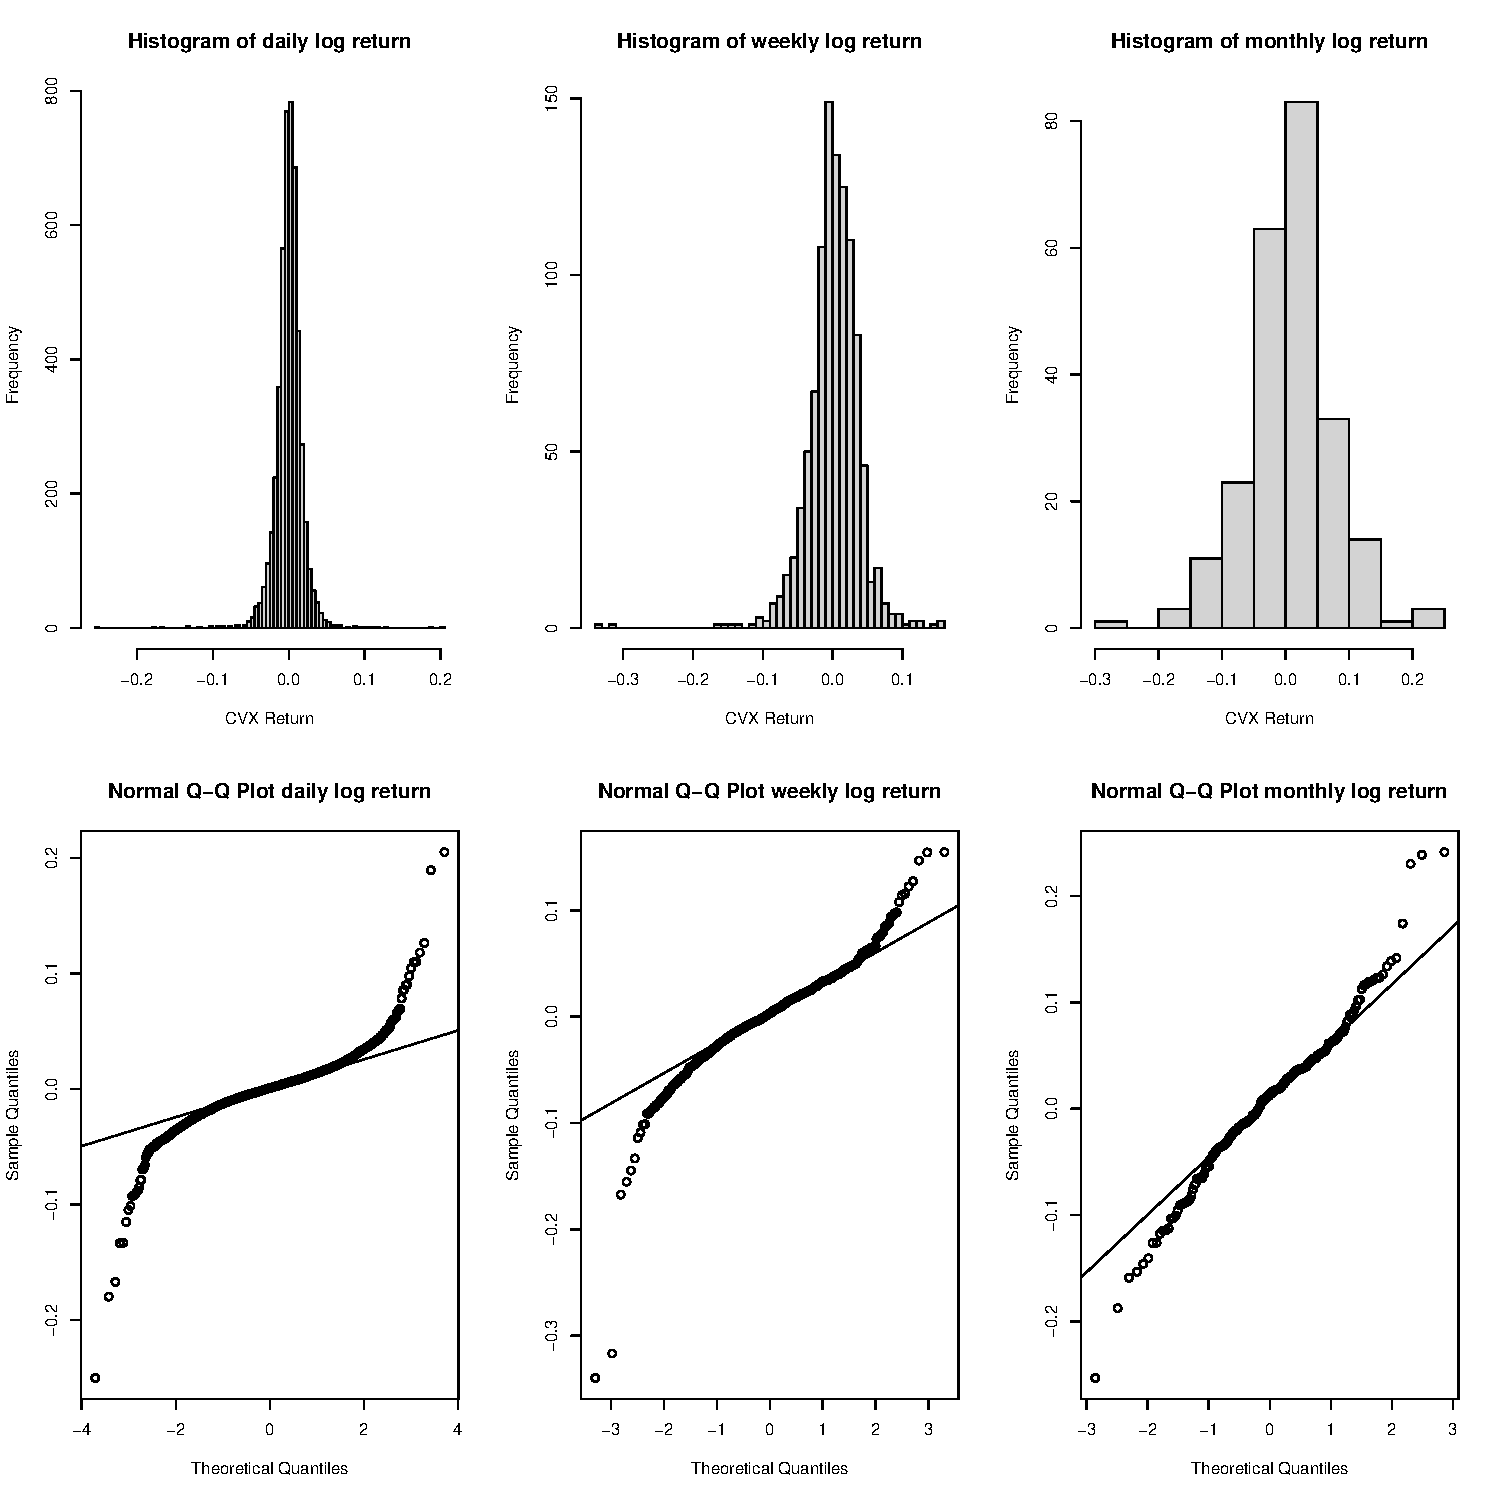
\includegraphics{homework_1_files/figure-pdf/unnamed-chunk-15-1.pdf}

}

\end{figure}

b)

In the daily log return quantile we can see the long and fat tails in
the sample quantile when compared to the standard normal. As the time of
return gets larger we the tails get less fat but still maintaining too
many outliers to be well fit by a normal distribution.

We can also see that each distribution has a left skew although it
becomes less severe in the monthly returns.

c)

\begin{Shaded}
\begin{Highlighting}[]
\CommentTok{\#Defining functions to compute skewness and kurtosis}
\NormalTok{Sk.fun }\OtherTok{\textless{}{-}} \ControlFlowTok{function}\NormalTok{(x) \{ }\DocumentationTok{\#\# function to compute skewness}
\FunctionTok{mean}\NormalTok{((x}\SpecialCharTok{{-}}\FunctionTok{mean}\NormalTok{(x))}\SpecialCharTok{\^{}}\DecValTok{3}\SpecialCharTok{/}\FunctionTok{sd}\NormalTok{(x)}\SpecialCharTok{\^{}}\DecValTok{3}\NormalTok{)}
\NormalTok{\}}
\NormalTok{Kur.fun }\OtherTok{\textless{}{-}} \ControlFlowTok{function}\NormalTok{(x)\{ }\DocumentationTok{\#\# function to compute kurtosis}
\FunctionTok{mean}\NormalTok{((x}\SpecialCharTok{{-}}\FunctionTok{mean}\NormalTok{(x))}\SpecialCharTok{\^{}}\DecValTok{4}\SpecialCharTok{/}\FunctionTok{sd}\NormalTok{(x)}\SpecialCharTok{\^{}}\DecValTok{4}\NormalTok{)}
\NormalTok{\}}
\end{Highlighting}
\end{Shaded}

\begin{Shaded}
\begin{Highlighting}[]
\NormalTok{daily\_skewness }\OtherTok{\textless{}{-}} \FunctionTok{Sk.fun}\NormalTok{(CVX\_returns[[}\DecValTok{1}\NormalTok{]])}
\NormalTok{daily\_kurtosis }\OtherTok{\textless{}{-}} \FunctionTok{Kur.fun}\NormalTok{(CVX\_returns[[}\DecValTok{1}\NormalTok{]])}
\NormalTok{daily\_shapiro\_wilk }\OtherTok{\textless{}{-}} \FunctionTok{shapiro.test}\NormalTok{((}\FunctionTok{as.numeric}\NormalTok{(CVX\_returns[[}\DecValTok{1}\NormalTok{]])))}

\NormalTok{weekly\_skewness }\OtherTok{\textless{}{-}} \FunctionTok{Sk.fun}\NormalTok{(}\FunctionTok{as.numeric}\NormalTok{(CVX\_returns[[}\DecValTok{2}\NormalTok{]]))}
\NormalTok{weekly\_kurtosis }\OtherTok{\textless{}{-}} \FunctionTok{Kur.fun}\NormalTok{(}\FunctionTok{as.numeric}\NormalTok{(CVX\_returns[[}\DecValTok{2}\NormalTok{]]))}
\NormalTok{weekly\_shapiro\_wilk }\OtherTok{\textless{}{-}} \FunctionTok{shapiro.test}\NormalTok{(}\FunctionTok{as.numeric}\NormalTok{(CVX\_returns[[}\DecValTok{2}\NormalTok{]]))}

\NormalTok{monthly\_skewness }\OtherTok{\textless{}{-}} \FunctionTok{Sk.fun}\NormalTok{(}\FunctionTok{as.numeric}\NormalTok{(CVX\_returns[[}\DecValTok{3}\NormalTok{]]))}
\NormalTok{monthly\_kurtosis }\OtherTok{\textless{}{-}} \FunctionTok{Kur.fun}\NormalTok{(}\FunctionTok{as.numeric}\NormalTok{(CVX\_returns[[}\DecValTok{3}\NormalTok{]]))}
\NormalTok{monthly\_shapiro\_wilk }\OtherTok{\textless{}{-}} \FunctionTok{shapiro.test}\NormalTok{(}\FunctionTok{as.numeric}\NormalTok{(CVX\_returns[[}\DecValTok{3}\NormalTok{]]))}

\FunctionTok{paste}\NormalTok{(}\StringTok{"Daily statistics: Skewness:"}\NormalTok{,daily\_skewness,}\StringTok{"Kurtosis:"}\NormalTok{,daily\_kurtosis)}
\end{Highlighting}
\end{Shaded}

\begin{verbatim}
[1] "Daily statistics: Skewness: -0.506884204015888 Kurtosis: 24.6939389714861"
\end{verbatim}

\begin{Shaded}
\begin{Highlighting}[]
\NormalTok{daily\_shapiro\_wilk}
\end{Highlighting}
\end{Shaded}

\begin{verbatim}

    Shapiro-Wilk normality test

data:  (as.numeric(CVX_returns[[1]]))
W = 0.87278, p-value < 2.2e-16
\end{verbatim}

\begin{Shaded}
\begin{Highlighting}[]
\FunctionTok{paste}\NormalTok{(}\StringTok{"Weekly statistics: Skewness:"}\NormalTok{,weekly\_skewness,}\StringTok{"Kurtosis:"}\NormalTok{,weekly\_kurtosis)}
\end{Highlighting}
\end{Shaded}

\begin{verbatim}
[1] "Weekly statistics: Skewness: -1.42259796733426 Kurtosis: 15.7761560268946"
\end{verbatim}

\begin{Shaded}
\begin{Highlighting}[]
\NormalTok{weekly\_shapiro\_wilk}
\end{Highlighting}
\end{Shaded}

\begin{verbatim}

    Shapiro-Wilk normality test

data:  as.numeric(CVX_returns[[2]])
W = 0.90397, p-value < 2.2e-16
\end{verbatim}

\begin{Shaded}
\begin{Highlighting}[]
\FunctionTok{paste}\NormalTok{(}\StringTok{"Monthly statistics: Skewness:"}\NormalTok{,monthly\_skewness,}\StringTok{"Kurtosis:"}\NormalTok{,}
\NormalTok{      monthly\_kurtosis)}
\end{Highlighting}
\end{Shaded}

\begin{verbatim}
[1] "Monthly statistics: Skewness: -0.0355891766527548 Kurtosis: 4.69414203147567"
\end{verbatim}

\begin{Shaded}
\begin{Highlighting}[]
\NormalTok{monthly\_shapiro\_wilk}
\end{Highlighting}
\end{Shaded}

\begin{verbatim}

    Shapiro-Wilk normality test

data:  as.numeric(CVX_returns[[3]])
W = 0.9743, p-value = 0.0002864
\end{verbatim}

The Shapiro-Wilk normality tests the following hypothesis with
\(H_0=Normaility\) and \(H_1=Non-Normality\) its test statistic is the
correlation between the sample quantile and the theoretical normal
quantile.

As the period of return gets larger we can see the test statistic for
the Shapiro Wilk test get larger, going from 0.87 for daily returns to
0.97 for monthly returns, the fit of the normal distribution gets better
as more return data is grouped. Despite, this the hypothesis of
normality is rejected for each period, agreeing with our visual
inspection of the normal qq-plots.

The skewness of the graph is moderately left skewed in the daily and
weekly return and is close to unskewed in the monthly return reflecting
some asymmetry in returns.

The kurtosis statistic gives us information that is harder to see in the
histograms. We see extreme kurtosis in the daily return a measure of
24.69, far greater than the normal distributions kurtosis of 3. This
indicates a lot of the weight in the data is in the center and tails. We
can also see the kurtosis approach 3 as the period of return gets
larger, with monthly return's kurtosis being 4.69. This reflects the
principle of aggregational gaussianity in financial return data.

7)

\begin{Shaded}
\begin{Highlighting}[]
\NormalTok{n }\OtherTok{=} \FunctionTok{length}\NormalTok{(SnP\_500\_dlr)}
\NormalTok{q\_grid }\OtherTok{=}\NormalTok{ (}\DecValTok{1}\SpecialCharTok{:}\NormalTok{n) }\SpecialCharTok{/}\NormalTok{ (n }\SpecialCharTok{+} \DecValTok{1}\NormalTok{)}
\NormalTok{df\_grid }\OtherTok{=} \DecValTok{2}\SpecialCharTok{:}\DecValTok{7}
\FunctionTok{par}\NormalTok{(}\AttributeTok{mfrow =} \FunctionTok{c}\NormalTok{(}\DecValTok{3}\NormalTok{,}\DecValTok{2}\NormalTok{))}
\ControlFlowTok{for}\NormalTok{(i }\ControlFlowTok{in} \DecValTok{1}\SpecialCharTok{:}\DecValTok{6}\NormalTok{)\{}
 \FunctionTok{qqplot}\NormalTok{(}\AttributeTok{y =} \FunctionTok{as.numeric}\NormalTok{(SnP\_500\_dlr), }\AttributeTok{x =} \FunctionTok{qt}\NormalTok{(q\_grid,df\_grid[i]),}
 \AttributeTok{main =} \FunctionTok{paste}\NormalTok{(}\StringTok{"S\&P 500 Normal QQ"}\NormalTok{, }\StringTok{", df = "}\NormalTok{, df\_grid[i]), }
 \AttributeTok{xlab =} \StringTok{"Theoretical Quantiles"}\NormalTok{, }\AttributeTok{ylab =} \StringTok{"Sample Quantiles"}\NormalTok{)}
  \FunctionTok{abline}\NormalTok{(}\FunctionTok{lm}\NormalTok{(}\FunctionTok{quantile}\NormalTok{(SnP\_500\_dlr, }\FunctionTok{c}\NormalTok{(}\FloatTok{0.25}\NormalTok{, }\FloatTok{0.75}\NormalTok{)) }\SpecialCharTok{\textasciitilde{}} 
             \FunctionTok{qt}\NormalTok{(}\FunctionTok{c}\NormalTok{(}\FloatTok{0.25}\NormalTok{, }\FloatTok{0.75}\NormalTok{), }\AttributeTok{df =}\NormalTok{ df\_grid[i])))}
\NormalTok{\}}
\end{Highlighting}
\end{Shaded}

\begin{figure}[H]

{\centering 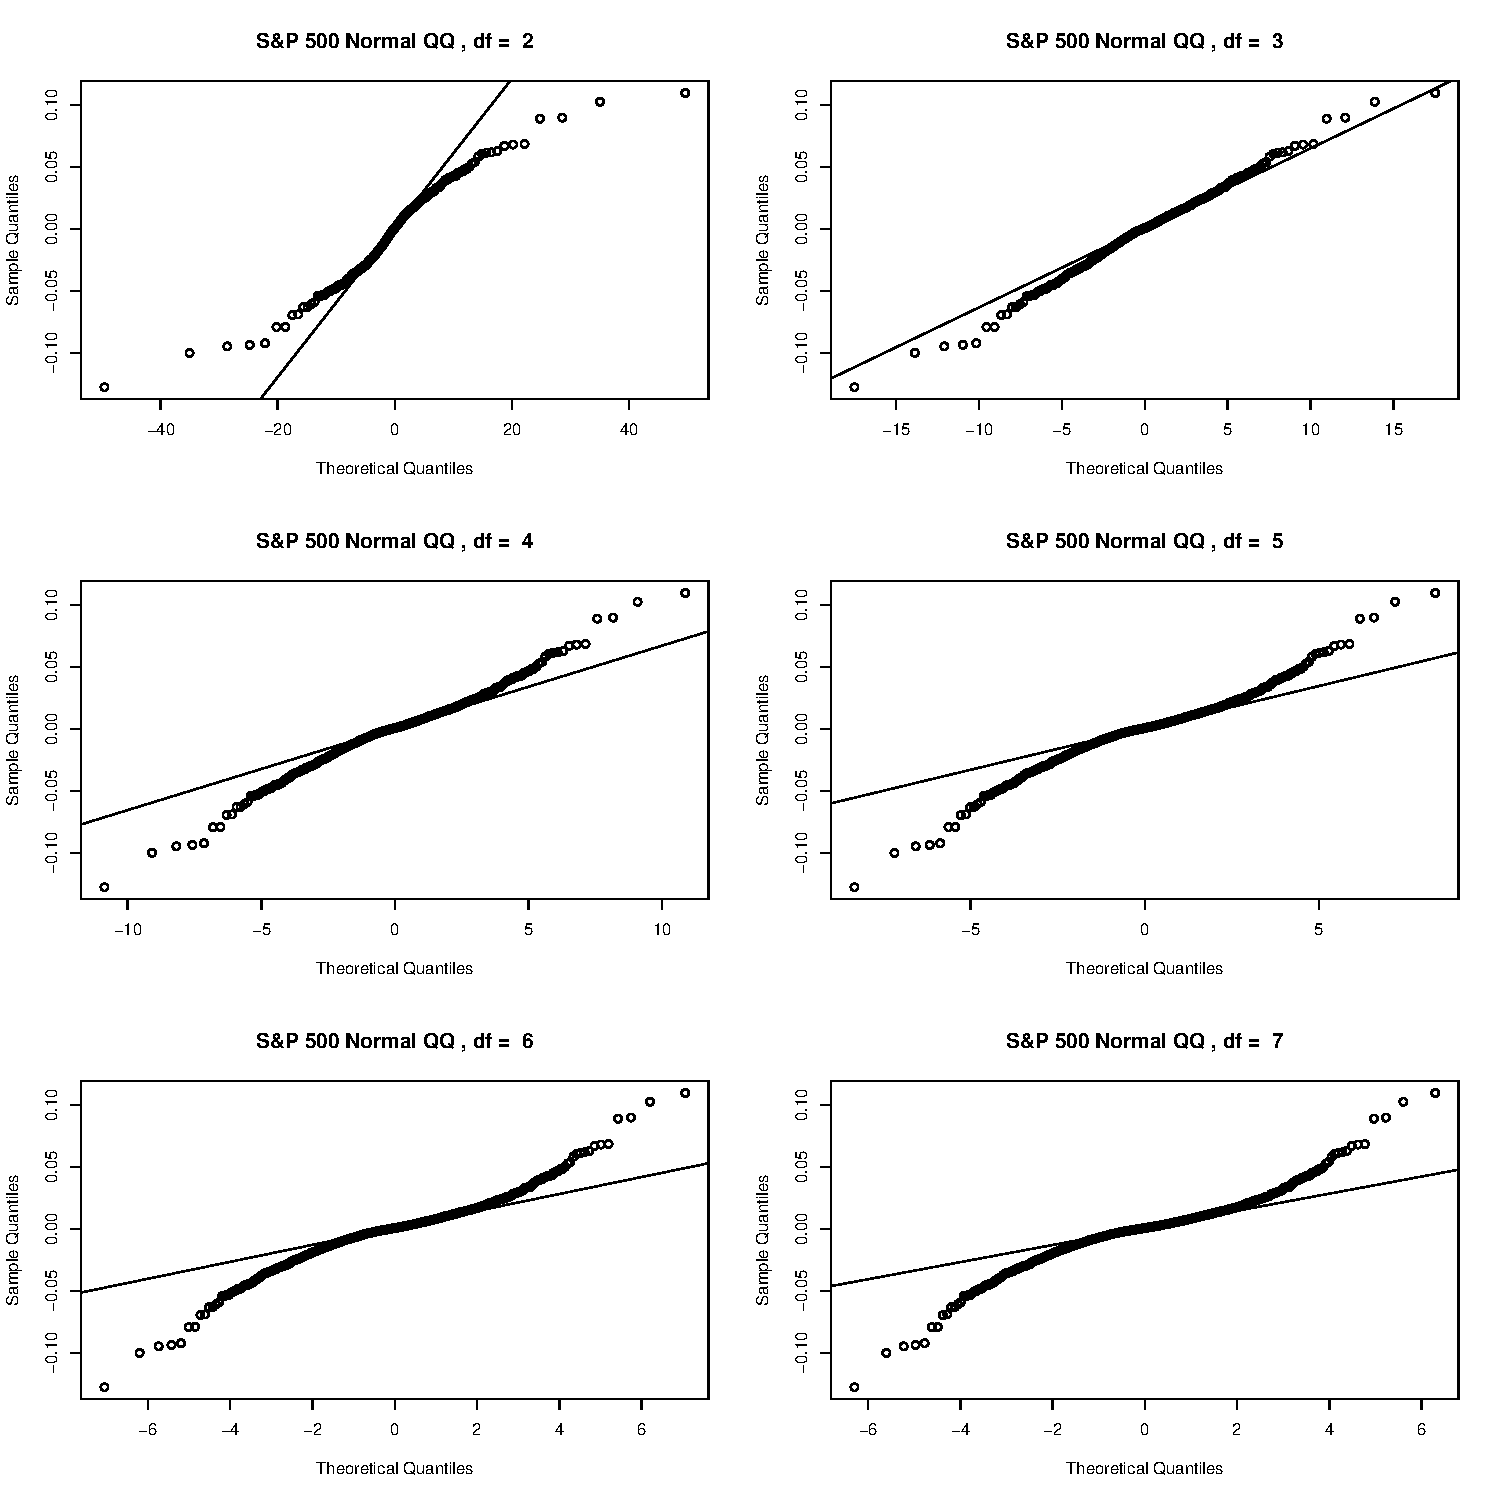
\includegraphics{homework_1_files/figure-pdf/unnamed-chunk-18-1.pdf}

}

\end{figure}

Problem 4)

The code q.grid = (1:n) / (n + 1) creates an evenly spaced out vector of
length n that avoids inputs of probability 0 and 1. The limit as p
approaches 0 equals negative infinity, similarly the limit as p
approaches 1 equals infinity. If we don't make this adjustment and just
equally spaced q.grid from 0 to 1 it would both the graph by making our
x axis way too large and it would be unreadable.

The code qt(q.grid, df = df{[}j{]}) (in my code
qt(q\_grid,df\_grid{[}i{]})) computes the quantiles of the t
distribution using the probability inputs of q.grid with a different
degree of freedom from the vector df\_grid with each loop.

Problem 5)

The best fitting distribution is the t distribution with degrees of
freedom equal to 3. The data closely follows the fitted line with only
slight deviation at the tails. The other choices of degrees of freedom
have clear issues in the tails with many fatter and longer than the
theoretical distribution.

Problem 6)

\begin{Shaded}
\begin{Highlighting}[]
\FunctionTok{library}\NormalTok{(}\StringTok{"fGarch"}\NormalTok{)}
\end{Highlighting}
\end{Shaded}

\begin{verbatim}
NOTE: Packages 'fBasics', 'timeDate', and 'timeSeries' are no longer
attached to the search() path when 'fGarch' is attached.

If needed attach them yourself in your R script by e.g.,
        require("timeSeries")
\end{verbatim}

\begin{verbatim}

Attaching package: 'fGarch'
\end{verbatim}

\begin{verbatim}
The following object is masked from 'package:TTR':

    volatility
\end{verbatim}

\begin{Shaded}
\begin{Highlighting}[]
\NormalTok{x}\OtherTok{=}\FunctionTok{seq}\NormalTok{(}\SpecialCharTok{{-}}\FloatTok{0.1}\NormalTok{, }\FloatTok{0.1}\NormalTok{,}\AttributeTok{by =} \FloatTok{0.001}\NormalTok{)}
\FunctionTok{par}\NormalTok{(}\AttributeTok{mfrow =} \FunctionTok{c}\NormalTok{(}\DecValTok{1}\NormalTok{, }\DecValTok{1}\NormalTok{))}
\NormalTok{df }\OtherTok{=} \DecValTok{3}
\NormalTok{mad\_t }\OtherTok{=} \FunctionTok{mad}\NormalTok{(SnP\_500\_dlr, }
            \AttributeTok{constant =} \FunctionTok{sqrt}\NormalTok{(df }\SpecialCharTok{/}\NormalTok{ (df}\SpecialCharTok{{-}} \DecValTok{2}\NormalTok{)) }\SpecialCharTok{/} \FunctionTok{qt}\NormalTok{(}\FloatTok{0.75}\NormalTok{, df))}
\FunctionTok{plot}\NormalTok{(}\FunctionTok{density}\NormalTok{(SnP\_500\_dlr), }\AttributeTok{lwd =} \DecValTok{2}\NormalTok{, }\AttributeTok{ylim =} \FunctionTok{c}\NormalTok{(}\DecValTok{0}\NormalTok{, }\DecValTok{60}\NormalTok{))}
\FunctionTok{lines}\NormalTok{(x, }\FunctionTok{dstd}\NormalTok{(x, }\AttributeTok{mean =} \FunctionTok{mean}\NormalTok{(SnP\_500\_dlr), }\AttributeTok{sd =}\NormalTok{ mad\_t, }\AttributeTok{nu =}\NormalTok{ df),}
 \AttributeTok{lty =} \DecValTok{5}\NormalTok{, }\AttributeTok{lwd =} \DecValTok{2}\NormalTok{, }\AttributeTok{col =} \StringTok{"red"}\NormalTok{)}
\FunctionTok{lines}\NormalTok{(x, }\FunctionTok{dnorm}\NormalTok{(x, }\AttributeTok{mean =} \FunctionTok{mean}\NormalTok{(SnP\_500\_dlr), }\AttributeTok{sd =} \FunctionTok{sd}\NormalTok{(SnP\_500\_dlr)),}
 \AttributeTok{lty =} \DecValTok{3}\NormalTok{, }\AttributeTok{lwd =} \DecValTok{4}\NormalTok{, }\AttributeTok{col =} \StringTok{"blue"}\NormalTok{)}
\FunctionTok{legend}\NormalTok{(}\StringTok{"topleft"}\NormalTok{, }\FunctionTok{c}\NormalTok{(}\StringTok{"KDE"}\NormalTok{, }\FunctionTok{paste}\NormalTok{(}\StringTok{"t: df = "}\NormalTok{,df), }\StringTok{"normal"}\NormalTok{),}
 \AttributeTok{lwd =} \FunctionTok{c}\NormalTok{(}\DecValTok{2}\NormalTok{, }\DecValTok{2}\NormalTok{, }\DecValTok{4}\NormalTok{), }\AttributeTok{lty =} \FunctionTok{c}\NormalTok{(}\DecValTok{1}\NormalTok{, }\DecValTok{5}\NormalTok{, }\DecValTok{3}\NormalTok{),}
 \AttributeTok{col =} \FunctionTok{c}\NormalTok{(}\StringTok{"black"}\NormalTok{, }\StringTok{"red"}\NormalTok{, }\StringTok{"blue"}\NormalTok{))}
\end{Highlighting}
\end{Shaded}

\begin{figure}[H]

{\centering 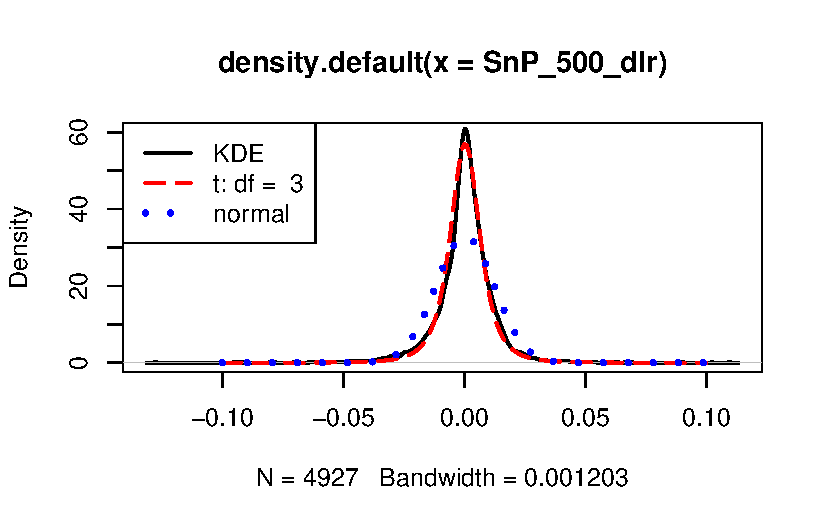
\includegraphics{homework_1_files/figure-pdf/unnamed-chunk-19-1.pdf}

}

\end{figure}

\begin{Shaded}
\begin{Highlighting}[]
\FunctionTok{par}\NormalTok{(}\AttributeTok{mfrow =} \FunctionTok{c}\NormalTok{(}\DecValTok{1}\NormalTok{,}\DecValTok{2}\NormalTok{))}

\FunctionTok{plot}\NormalTok{(}\FunctionTok{density}\NormalTok{(SnP\_500\_dlr), }\AttributeTok{lwd =} \DecValTok{2}\NormalTok{, }\AttributeTok{ylim =} \FunctionTok{c}\NormalTok{(}\DecValTok{0}\NormalTok{, }\DecValTok{1}\NormalTok{), }\AttributeTok{xlim =} \FunctionTok{c}\NormalTok{(}\SpecialCharTok{{-}}\NormalTok{.}\DecValTok{1}\NormalTok{, }\SpecialCharTok{{-}}\FloatTok{0.03}\NormalTok{),}
     \AttributeTok{main =} \StringTok{"Left Tail"}\NormalTok{)}
\FunctionTok{lines}\NormalTok{(x, }\FunctionTok{dstd}\NormalTok{(x, }\AttributeTok{mean =} \FunctionTok{mean}\NormalTok{(SnP\_500\_dlr), }\AttributeTok{sd =}\NormalTok{ mad\_t, }\AttributeTok{nu =}\NormalTok{ df),}
 \AttributeTok{lty =} \DecValTok{5}\NormalTok{, }\AttributeTok{lwd =} \DecValTok{2}\NormalTok{, }\AttributeTok{col =} \StringTok{"red"}\NormalTok{)}
\FunctionTok{lines}\NormalTok{(x, }\FunctionTok{dnorm}\NormalTok{(x, }\AttributeTok{mean =} \FunctionTok{mean}\NormalTok{(SnP\_500\_dlr), }\AttributeTok{sd =} \FunctionTok{sd}\NormalTok{(SnP\_500\_dlr)),}
 \AttributeTok{lty =} \DecValTok{3}\NormalTok{, }\AttributeTok{lwd =} \DecValTok{4}\NormalTok{, }\AttributeTok{col =} \StringTok{"blue"}\NormalTok{)}
\FunctionTok{legend}\NormalTok{(}\StringTok{"topleft"}\NormalTok{, }\FunctionTok{c}\NormalTok{(}\StringTok{"KDE"}\NormalTok{, }\FunctionTok{paste}\NormalTok{(}\StringTok{"t: df = "}\NormalTok{,df), }\StringTok{"normal"}\NormalTok{),}
 \AttributeTok{lwd =} \FunctionTok{c}\NormalTok{(}\DecValTok{2}\NormalTok{, }\DecValTok{2}\NormalTok{, }\DecValTok{4}\NormalTok{), }\AttributeTok{lty =} \FunctionTok{c}\NormalTok{(}\DecValTok{1}\NormalTok{, }\DecValTok{5}\NormalTok{, }\DecValTok{3}\NormalTok{),}
 \AttributeTok{col =} \FunctionTok{c}\NormalTok{(}\StringTok{"black"}\NormalTok{, }\StringTok{"red"}\NormalTok{, }\StringTok{"blue"}\NormalTok{))}

\FunctionTok{plot}\NormalTok{(}\FunctionTok{density}\NormalTok{(SnP\_500\_dlr), }\AttributeTok{lwd =} \DecValTok{2}\NormalTok{, }\AttributeTok{ylim =} \FunctionTok{c}\NormalTok{(}\DecValTok{0}\NormalTok{, }\DecValTok{1}\NormalTok{), }\AttributeTok{xlim =} \FunctionTok{c}\NormalTok{(}\FloatTok{0.03}\NormalTok{, }\FloatTok{0.1}\NormalTok{),}
     \AttributeTok{main =} \StringTok{"Right tail"}\NormalTok{)}
\FunctionTok{lines}\NormalTok{(x, }\FunctionTok{dstd}\NormalTok{(x, }\AttributeTok{mean =} \FunctionTok{mean}\NormalTok{(SnP\_500\_dlr), }\AttributeTok{sd =}\NormalTok{ mad\_t, }\AttributeTok{nu =}\NormalTok{ df),}
 \AttributeTok{lty =} \DecValTok{5}\NormalTok{, }\AttributeTok{lwd =} \DecValTok{2}\NormalTok{, }\AttributeTok{col =} \StringTok{"red"}\NormalTok{)}
\FunctionTok{lines}\NormalTok{(x, }\FunctionTok{dnorm}\NormalTok{(x, }\AttributeTok{mean =} \FunctionTok{mean}\NormalTok{(SnP\_500\_dlr), }\AttributeTok{sd =} \FunctionTok{sd}\NormalTok{(SnP\_500\_dlr)),}
 \AttributeTok{lty =} \DecValTok{3}\NormalTok{, }\AttributeTok{lwd =} \DecValTok{4}\NormalTok{, }\AttributeTok{col =} \StringTok{"blue"}\NormalTok{)}
\FunctionTok{legend}\NormalTok{(}\StringTok{"topleft"}\NormalTok{, }\FunctionTok{c}\NormalTok{(}\StringTok{"KDE"}\NormalTok{, }\FunctionTok{paste}\NormalTok{(}\StringTok{"t: df = "}\NormalTok{,df), }\StringTok{"normal"}\NormalTok{),}
 \AttributeTok{lwd =} \FunctionTok{c}\NormalTok{(}\DecValTok{2}\NormalTok{, }\DecValTok{2}\NormalTok{, }\DecValTok{4}\NormalTok{), }\AttributeTok{lty =} \FunctionTok{c}\NormalTok{(}\DecValTok{1}\NormalTok{, }\DecValTok{5}\NormalTok{, }\DecValTok{3}\NormalTok{),}
 \AttributeTok{col =} \FunctionTok{c}\NormalTok{(}\StringTok{"black"}\NormalTok{, }\StringTok{"red"}\NormalTok{, }\StringTok{"blue"}\NormalTok{))}
\end{Highlighting}
\end{Shaded}

\begin{figure}[H]

{\centering 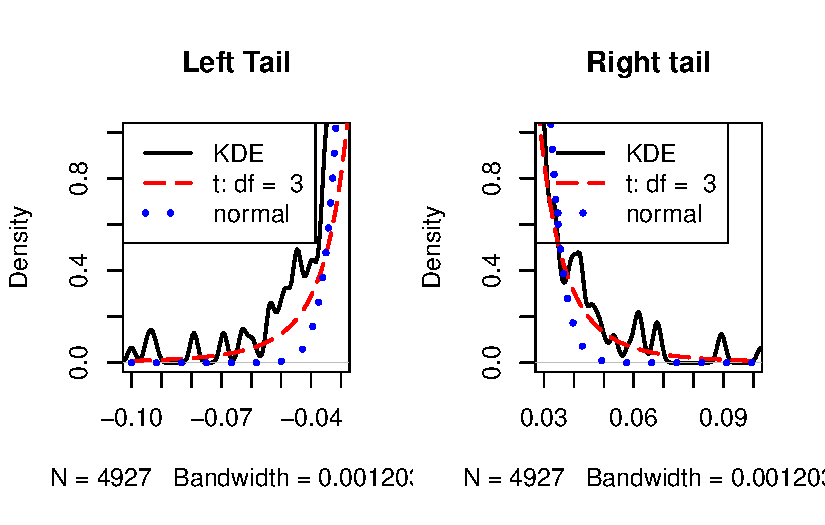
\includegraphics{homework_1_files/figure-pdf/unnamed-chunk-20-1.pdf}

}

\end{figure}

The t distribution with degrees of freedom of 3 does a great job of
fitting the return data. Looking at the center of the distribution we
can see how closely it follows the peak of the density estimate. In the
tails, we are very zoomed in so we can see many peaks and valleys of the
KDE but the t distribution does pretty well here too.

The normal distribution on the other hand does a very poor job. The peak
is far lower than the KDE and the density dissipates in the tail far
earlier than the return data.



\end{document}
